\documentclass[12pt]{beamer}

\mode<presentation> {\usetheme{metropolis}}

\usepackage{mathtools}
\usepackage{graphicx}
\usepackage{booktabs} % Allows the use of \toprule, \midrule and \bottomrule in tables

%----------------------------------------------------------------------------------------
%	TITLE PAGE
%----------------------------------------------------------------------------------------

\title[Intro to ML and AI]{Matrix Project On Coordinate Geometry}

\author{Sai Harsha Kottapalli and Abhishek Agarwal}
\institute[IITH]
{
Indian Institute of Technology Hyderabad
\medskip
}
\date{February 14, 2019}

\begin{document}

\begin{frame}
\titlepage
\end{frame}

\begin{frame}
\frametitle{Index}
\tableofcontents
\end{frame}

\section{Problem Statement}

\begin{frame}
\frametitle{Problem Statement}
$\textbf{P}$ and $\textbf{Q}$ are two distinct points on the parabola
\[
\textbf{x}^T
\begin{bmatrix}
    0 & 0\\
    0 & 1\\  
\end{bmatrix}
\textbf{x}  -  
\begin{bmatrix}
    4\\
    0\\  
\end{bmatrix}
\textbf{x} = 0
\]
with parameters $t$ and $t_1$ respectively.  If the normal at $\textbf{P} $ passes through $\textbf{Q}$, then find 
the minimum value of $t_1^2$.
\end{frame}

%------------------------------------------------
\section{Steps to solve the problem}
%------------------------------------------------

\begin{frame}
\frametitle{Steps}
\begin{itemize}
\item<1-5> Find the constants of the parabola
\item<2-5> Find Slope of tangent
\item<3-5> Find slope of Normal
\item<4-5> Write eqn of Normal using slope and parametric Point
\item<5> Minimise as a function of parameter of point P
\end{itemize}
\end{frame}

%------------------------------------------------
\section{Solution}
%------------------------------------------------

\begin{frame}
\frametitle{Solution}
\begin{itemize}
\item<1-4> Given equation:
\[
\textbf{x}^T
\begin{bmatrix}
    0 & 0\\
    0 & 1\\  
\end{bmatrix}
\textbf{x}  -  
\begin{bmatrix}
    4\\
    0\\  
\end{bmatrix}
\textbf{x} = 0
\] \\
\item<2-4> Since, 3 entries of the 2x2 matrix is 0, the parabola is of the standard form (i.e.) \[ y^2 = 4ax\]
\item<3-4> Coefficient of x = 4a
\item<4> a = 1
\end{itemize}
\end{frame}

%------------------------------------------------

\begin{frame}
\frametitle{Solution Contd..}
\begin{itemize}
\item<1-3> Parametric form of points of parabola: 
\[
\begin{bmatrix}
    t^2\\
    2t\\  
\end{bmatrix}
\]
\item<2-3> Differentiate the equation and substitute $\frac{dy}{dx}$ = m (the slope of the tangent)
\item<3> $\frac{d\textbf{x}}{dx} = 
\begin{bmatrix}
    1 & m
\end{bmatrix}^T$
\end{itemize}
\end{frame}

%------------------------------------------------

\begin{frame}
\frametitle{Solution Contd..}
\begin{itemize}
\item<1-2>
\[
\begin{bmatrix}
    1\\
    m\\  
\end{bmatrix}^T
\begin{bmatrix}
    0 & 0\\
    0 & 1\\  
\end{bmatrix}
\textbf{x} + 
\textbf{x}^T
\begin{bmatrix}
    0 & 0\\
    0 & 1\\  
\end{bmatrix}
\begin{bmatrix}
    1\\
    m\\  
\end{bmatrix} - 
\begin{bmatrix}
    4\\
    0\\  
\end{bmatrix}^T
\begin{bmatrix}
    1\\
    m\\  
\end{bmatrix} = 0
\]
\item<2> Now, use the parametric form of \textbf{x} (i.e.)
\[
\textbf{x} = 
\begin{bmatrix}
    t^2\\
    2t\\  
\end{bmatrix}
\]
\end{itemize}
\end{frame}


%------------------------------------------------

\begin{frame}
\frametitle{Solution Contd..}
\begin{itemize}
\item<1-4>
\[
\begin{bmatrix}
    1 & m  
\end{bmatrix}
\begin{bmatrix}
    0\\
    2t\\  
\end{bmatrix} + 
\begin{bmatrix}
    t^2 & 2t  
\end{bmatrix}
\begin{bmatrix}
    0\\
    m\\  
\end{bmatrix} - 4 = 0
\]
\item<2-4> 2mt + 2mt - 4 = 0
\item<3-4> 4mt - 4 = 0
\item<4> m = $\frac{1}{t}$
\end{itemize}
\end{frame}


%------------------------------------------------

\begin{frame}
\frametitle{Solution Contd..}
\begin{itemize}
\item<1-3> We know that, Two lines are perpendicular if the product of their slopes is -1.
\item<2-3> Slope of normal at point \textbf{p}: $m_N$ = -t
\item<3> We calculate the equation of the line through P with slope = $m_N$
\end{itemize}
\end{frame}

%------------------------------------------------

\begin{frame}
\frametitle{Solution Contd..}
\begin{itemize}
\item<1-4> Note: \textbf{p} = $( x_1, y_1 )$ = $( t^2, 2t )$
\item<2-4>
\[
\begin{bmatrix}
    -m & 1  
\end{bmatrix}
\begin{bmatrix}
    x\\
    y\\  
\end{bmatrix} = 
\begin{bmatrix}
    -m & 1  
\end{bmatrix}
\begin{bmatrix}
    x_1\\
    y_1\\  
\end{bmatrix}
\]
\item<3-4>
\[
\begin{bmatrix}
    t & 1  
\end{bmatrix}
\begin{bmatrix}
    x\\
    y\\  
\end{bmatrix} = 
\begin{bmatrix}
    t & 1  
\end{bmatrix}
\begin{bmatrix}
    t^2\\
    2t\\  
\end{bmatrix}
\]
\item<4> \[
\begin{bmatrix}
    t & 1  
\end{bmatrix}
\begin{bmatrix}
    x\\
    y\\  
\end{bmatrix} = 
t^3 + 2t
\]
\end{itemize}
\end{frame}

%------------------------------------------------

\begin{frame}
\frametitle{Solution Contd..}
\begin{itemize}
\item<1-5> Now, Let Q: $( t_1^2, 2t_1 )$
\item<2-5> Then, We have,
\[
\begin{bmatrix}
    t & 1  
\end{bmatrix}
\begin{bmatrix}
    t_1^2\\
    2t_1\\  
\end{bmatrix} = 
t^3 + 2t
\]
\item<3-5> \[
2t_1 + tt_1^2 = t^3 + 2t 
\]
\item<4-5>
\[
-2(t - t_1) = t(t_1 + t)(t - t_1)
\]
\item<5>
\[
t_1 = -t - \frac{2}{t}
\]
\end{itemize}
\end{frame}


%------------------------------------------------

\begin{frame}
\frametitle{Solution Contd..}
\begin{itemize}
\item<1-5>
Squaring the previous equation, we get,
\[
t_1^2 = t^2 + \frac{4}{t^2} + 4
\]
\item<2-5> To solve above equation we use the property:\\
Arithmetic Mean $\geq$ Geometric Mean on $t^2 + \frac{4}{t^2}$
\item<3-5> A.M $\geq$ G.M. $\implies$ $t^2 + \frac{4}{t^2}$ $\geq$ 2$\sqrt{4}$ = 4
\item<4-5> $t_1^2 \geq$ 4 + 4 = 8
\item Note: $t_1 \neq 0$ because, in this case the normal will never intersect the parabola.
\item<5> $\therefore$ The Minimum possible value of $t_1^2$ is 8.
\end{itemize}
\end{frame}

%------------------------------------------------
\section{Figures}
%------------------------------------------------

\begin{frame}
\frametitle{Bounds of $t_1$ and $t_1^2$}
\begin{figure}
\centering
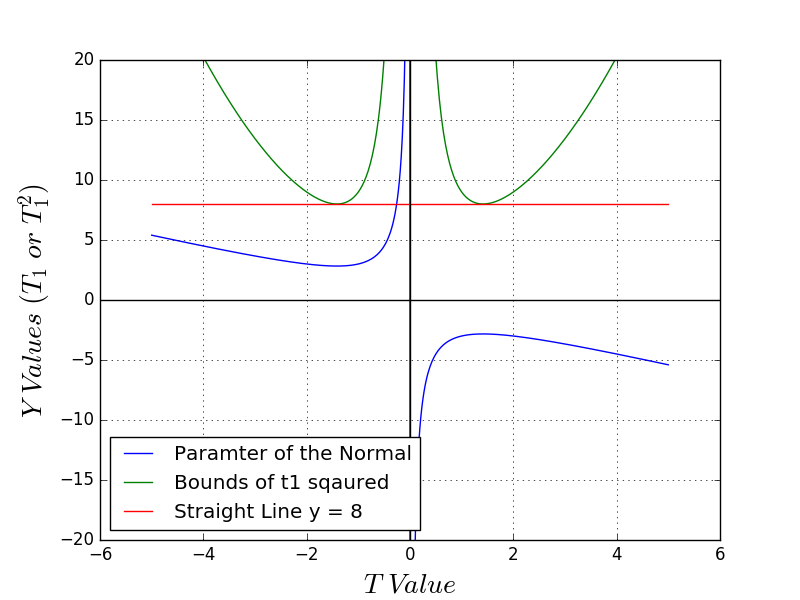
\includegraphics[scale=0.5]{/home/harsha/Documents/gitLab/Assignments/4th_semester/Intro_to_AI_and_ML/matrix-project/figures/minimisation.png}
\label{Bounds of $t_1$ and $t_1^2$}
\end{figure}
\end{frame}

%------------------------------------------------

\begin{frame}
\frametitle{Normal at minimum $t_1^2$}
\begin{figure}
\centering
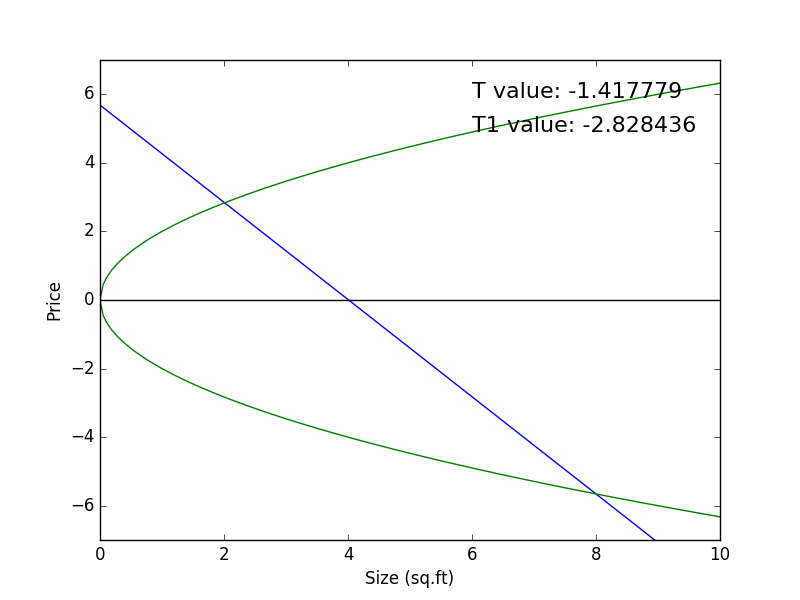
\includegraphics[scale=0.5]{/home/harsha/Documents/gitLab/Assignments/4th_semester/Intro_to_AI_and_ML/matrix-project/figures/frames/115.png}
\label{Normal at minimum $t_1^2$}
\end{figure}
\end{frame}

%------------------------------------------------

\begin{frame}
\frametitle{$t_1^2$ = 0}
\begin{figure}
\centering
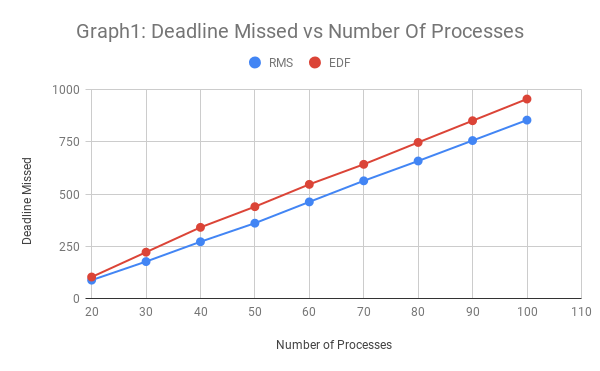
\includegraphics[scale=0.5]{/home/harsha/Documents/gitLab/Assignments/4th_semester/Intro_to_AI_and_ML/matrix-project/figures/frames/1.png}
\label{$t_1^2 = 0$}
\end{figure}
\end{frame}

%------------------------------------------------

\begin{frame}
\Huge{\centerline{The End}}
\end{frame}

%----------------------------------------------------------------------------------------

\end{document} 